\documentclass[11pt,a4paper]{article}

\usepackage[utf8]{inputenc} 
\usepackage[T1]{fontenc} 
\usepackage{lmodern}
\usepackage[margin=2cm]{geometry}
\usepackage[german]{babel}
\usepackage{amsmath} 
\usepackage{graphicx} 
\usepackage{booktabs}
\usepackage{hyperref}
\hypersetup{
    colorlinks,
    citecolor=red,
    filecolor=black,
    linkcolor=black!20!blue!90!,
    urlcolor=black} 
\usepackage{nicefrac}
\usepackage[table]{xcolor}
\usepackage{tocloft}

\setlength{\parindent}{0pt}
\setlength{\parskip}{1ex plus 0.5ex minus 0.5ex}

\definecolor{incolor}{rgb}{0.0, 0.0, 0.5}

\hbadness=99999

\newcommand{\refpy}[1]{Siehe Anhang: \textit{Rechnungen in Python} (\texttt{{\color{incolor}In [{\color{incolor}#1}]}})}
\newcommand\dif{\mathop{}\!\mathrm{d}}
\newcommand{\halftime}[4]{\begin{figure}[h]
\begin{minipage}{.#1\textwidth}#3\end{minipage}\begin{minipage}{.#2\textwidth}
\centering
#4\end{minipage}
\end{figure}}
\renewcommand{\vec}{\boldsymbol}

\begin{document}

{
\centering 
\large 
Physiklabor für Anf\"anger*innen \\
Ferienpraktikum im Sommersemester 2018 \\[4mm]
\textbf{\LARGE 
Versuch 14: Streuversuch
} \\[3mm]
(durchgef\"uhrt am 01.10.2018 bei Julia M\"uller) \\
Andréz Gockel, Patrick M\"unnich\\
\today \\[10mm]
}

\vspace{50pt}
\tableofcontents
\vspace{22pt}
\listoftables
\vspace{22pt}
\listoffigures
\pagebreak

\phantom{lol}
\thispagestyle{empty}
\pagebreak

\section{Ziel des Versuchs}

Das Ziel dieses Versuchs ist es, experimentell die Streuung von Teilchen zu visualisieren, in dem man Kugeln auf ein Target schie\ss t und die Auftreffpunkte betrachtet. Hiermit wird dann mit der Abh\"angigkeit des Streuwinkels vom Sto\ss parameter der Durchmesser des Targets bestimmt.

\section{Theorie}

Wird eine Kugel mit Radius $r$ auf eine festgehaltene Kugel mit Radius $R$, auch ,,Target'' genannt, gescho\ss en, so wird sie mit dem Streuwinkel $\theta$ gestreut. $\theta$ h\"angt hier vom Sto\ss parameter $b$ ab. Zum genaueren Verst\"andnis muss eine Skizze angebracht werden:

% 2.7 

Hierzu gelten folgende Formeln:

% change overline to curved

\begin{equation}
\overline{CE}=\overline{BD}=s\arcsin\frac{b}{s}\approx b\label{eq:1}
\end{equation}
\begin{equation}
\theta=\frac{\overline{AD}}{s}\approx\frac{\overline{AB}-b}{s}\label{eq:2}
\end{equation}
\begin{equation}
\sin\beta=\frac{b}{r+R}\label{eq:3}
\end{equation}

Au\ss erdem k\"onnen wir unser $\theta$ folgenderma\ss en ausdr\"ucken:
\begin{equation}
\theta=\frac{B}{s}\label{eq:4}
\end{equation}

\section{Aufbau}

\halftime{5}{5}{In diesem Versuch sind ein Streuapparat mit Plexi\-glasdeckel, eine Rolle druckempfindliches Papier, eine Schachtel mit Metallkugeln und ein Bandma\ss\ vorhanden. Der Streuapparat besteht aus einem Zylinder mit einer dran befestigten Schu\ss\-apparatur, welche mit Luftdruck funktioniert.}{\fbox{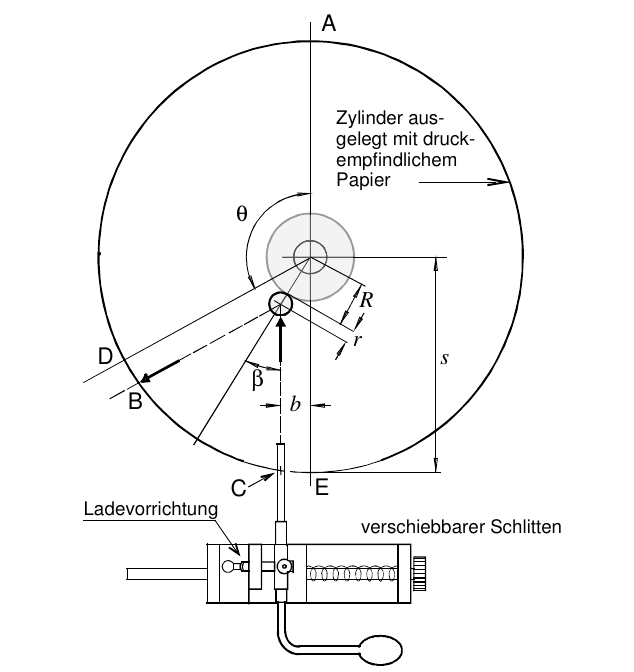
\includegraphics[width=0.5\textwidth]{aufbau.png}}
   \renewcommand\thefigure{2}
\caption{Versuchsaufbau. \cite{Anleitung}}
\label{Pic:2}}

\section{Durchführung}

% describe exp.
Man beginnt damit, dass das Papier an die Innenwand des Zylinder des Streuapparats gesteckt wird. Wichtig ist hier nat\"urlich, dass die druckempfindliche Seite nach innen zeigen muss.

Es werden dann f\"ur verschiedene Sto\ss parameter $b$, welche durch Bewegen des Schu\ss ger\"ats eingestellt werden, die Kugeln alle an das Target innerhalb des Streuapparats gescho\ss en. Sind alle Kugeln gescho\ss en, so wird der Sto\ss parameter ge\"andert. Zu beachten ist, dass man sowohl von rechts als auch von links schie\ss en muss.

\section{Auswertung}

F\"ur die Auswertung muss zuerst der Papierstreifen entfernt werden. Man betrachtet die Aufsto\ss punkte und mittelt sie. Hierzu beginnt man graphisch und findet rechts und links Grenzen, sodass 68\% der Punkte innerhalb der Grenzen liegen. Danach geht man analytisch vor und berechnet mit
\begin{equation}
\bar{x}=\frac{\sum_{i=1}^n x_i}{n}\label{mean}
\end{equation}
die Mittelwerte und mit
\begin{equation}
s_{\bar{x}}=\frac{{s_x}}{\sqrt{n}}\label{meanstd}
\end{equation}
deren Unsicherheiten. Wir erhalten damit folgende Werte:

\begin{table}[h]
\centering
\caption{Gemittelte Datenpunkte} \vspace{11pt}
$\begin{array}{l}
\textrm{Unsicherheiten:}\\
\textrm{B: } \pm 0.1 \textrm{cm}\\
\textrm{Position: } \pm 0.05 \textrm{cm}\\
\end{array}$
\begin{tabular}{ccc}
\toprule
\textrm{Messreihe} & \textrm{Position}/\textrm{cm} & \textrm{B}/\textrm{cm} \\
\midrule 
1 & 109.00 & 87.8 \\
2 & 108.00 & 65.0 \\
3 & 108.50 & 77.4 \\
4 & 107.50 & 49.4\\
5 & 111.50 & 64.5 \\
6 & 111.00 & 75.7\\
7 & 112.00 & 55.1 \\
8 & 111.75 & 50.2 \\
9 & 111.25 & 70.0 \\
10 & 109.25 & 70.25 \\ 
\bottomrule
\end{tabular}
\phantom{$\begin{array}{l}
\textrm{Unsicherheiten:}\\
\textrm{B: } \pm 0.1 \textrm{cm}\\
\textrm{Position: } \pm 0.05 \textrm{cm}\\
\end{array}$}
\label{Tab:1}
\end{table}

Um unsere Werte aufzutragen und den Radius $R$ zu bestimmen berechnen wir noch mit (\ref{eq:4}) die Werte f\"ur $\theta$. Wir verwenden f\"ur $s$ unser bestimmter Radius des zylindrischen Streuapparats von $(63.8\pm0.5)$\,cm und die eben berechneten Werte f\"ur die Positionen.

Um den Fehler unserer $\theta$ zu berechnen nutzen wir:
\[
\frac{\partial\theta}{\partial b}=\frac{1}{s}
\]
\[
\frac{\partial\theta}{\partial s}=-\frac{b}{s^2}
\]
\[
\Delta\theta=\sqrt{\left(\frac{\partial\theta}{\partial b}\Delta b\right)^2+\left(\frac{\partial\theta}{\partial s}\Delta s\right)^2}
\]

\pagebreak

Wir erhalten als Werte:

\begin{table}[h]
\centering
\caption{Werte f\"ur $\theta$} \vspace{11pt}
\begin{tabular}{ccc}
\toprule
\textrm{Messreihe} & \textrm{Position}/\textrm{cm} & $\theta$ /\textrm{rad} \\
\midrule 
1 & 109.00 & $2.75\pm0.02$ \\
2 & 108.00 & $2.03\pm0.02$ \\
3 & 108.50 & $2.43\pm0.02$ \\
4 & 107.50 & $1.55\pm0.01$\\
5 & 111.50 & $2.02\pm0.02$ \\
6 & 111.00 & $2.37\pm0.02$\\
7 & 112.00 & $1.73\pm0.01$ \\
8 & 111.75 & $1.57\pm0.01$ \\
9 & 111.25 & $2.19\pm0.02$ \\
10 & 109.25 & $2.20\pm0.02$ \\ 
\bottomrule
\end{tabular}
\label{Tab:2}
\end{table}

Wir k\"onnen jetzt also unsere Werte von $b$ gegen $\cos\left(\frac{\theta}{2}\right)$ auftragen. Wir f\"uhren aber zuerst noch eine lineare Regression durch. Da unsere zehnte Messung stark von den anderen Messungen dieser Messreihe abweicht, lassen wir diese raus. Aus unseren Formeln f\"ur die lineare Regression f\"ur ein Polynom der Form $y=ax+b$,

\begin{equation}
a=\frac{n\sum x_iy_i-\sum x_i\sum y_i}{n\sum x_i^2-(\sum x_i)^2}
\end{equation}
\begin{equation}
\Delta a=s\sqrt{\frac{n}{n\sum x_i^2-(\sum x_i)^2}},
\end{equation}
\begin{equation}
b=\frac{\sum x_i^2\sum y_i-\sum x_i\sum x_iy_i}{n\sum x_i^2-(\sum x_i)^2}
\end{equation}
\begin{equation}
\Delta b=s\sqrt{\frac{\sum x_i^2}{n\sum x_i^2-(\sum x_i)^2}}
\end{equation}
\begin{equation}
s=\sqrt{\frac{1}{n-2}\sum^n_{i=1}[y_i-(a+bx_i)]^2},
\end{equation}
interessiert uns eigentlich nur die Steigung $a$. Wir erhalten mit unserer Rechnung
\[a_{links}=-0.35\pm0.01\]
\[a_{rechts}=0.32\pm0.07\]

Zur Vervollst"andigung noch die $b$-Werte:
\[b_{links}=38\pm1\]
\[b_{rechts}=-35\pm8\]

\pagebreak

Das resultierende Bild sieht dann folgenderma\ss en aus:

\begin{figure}[h]
\centering
\fbox{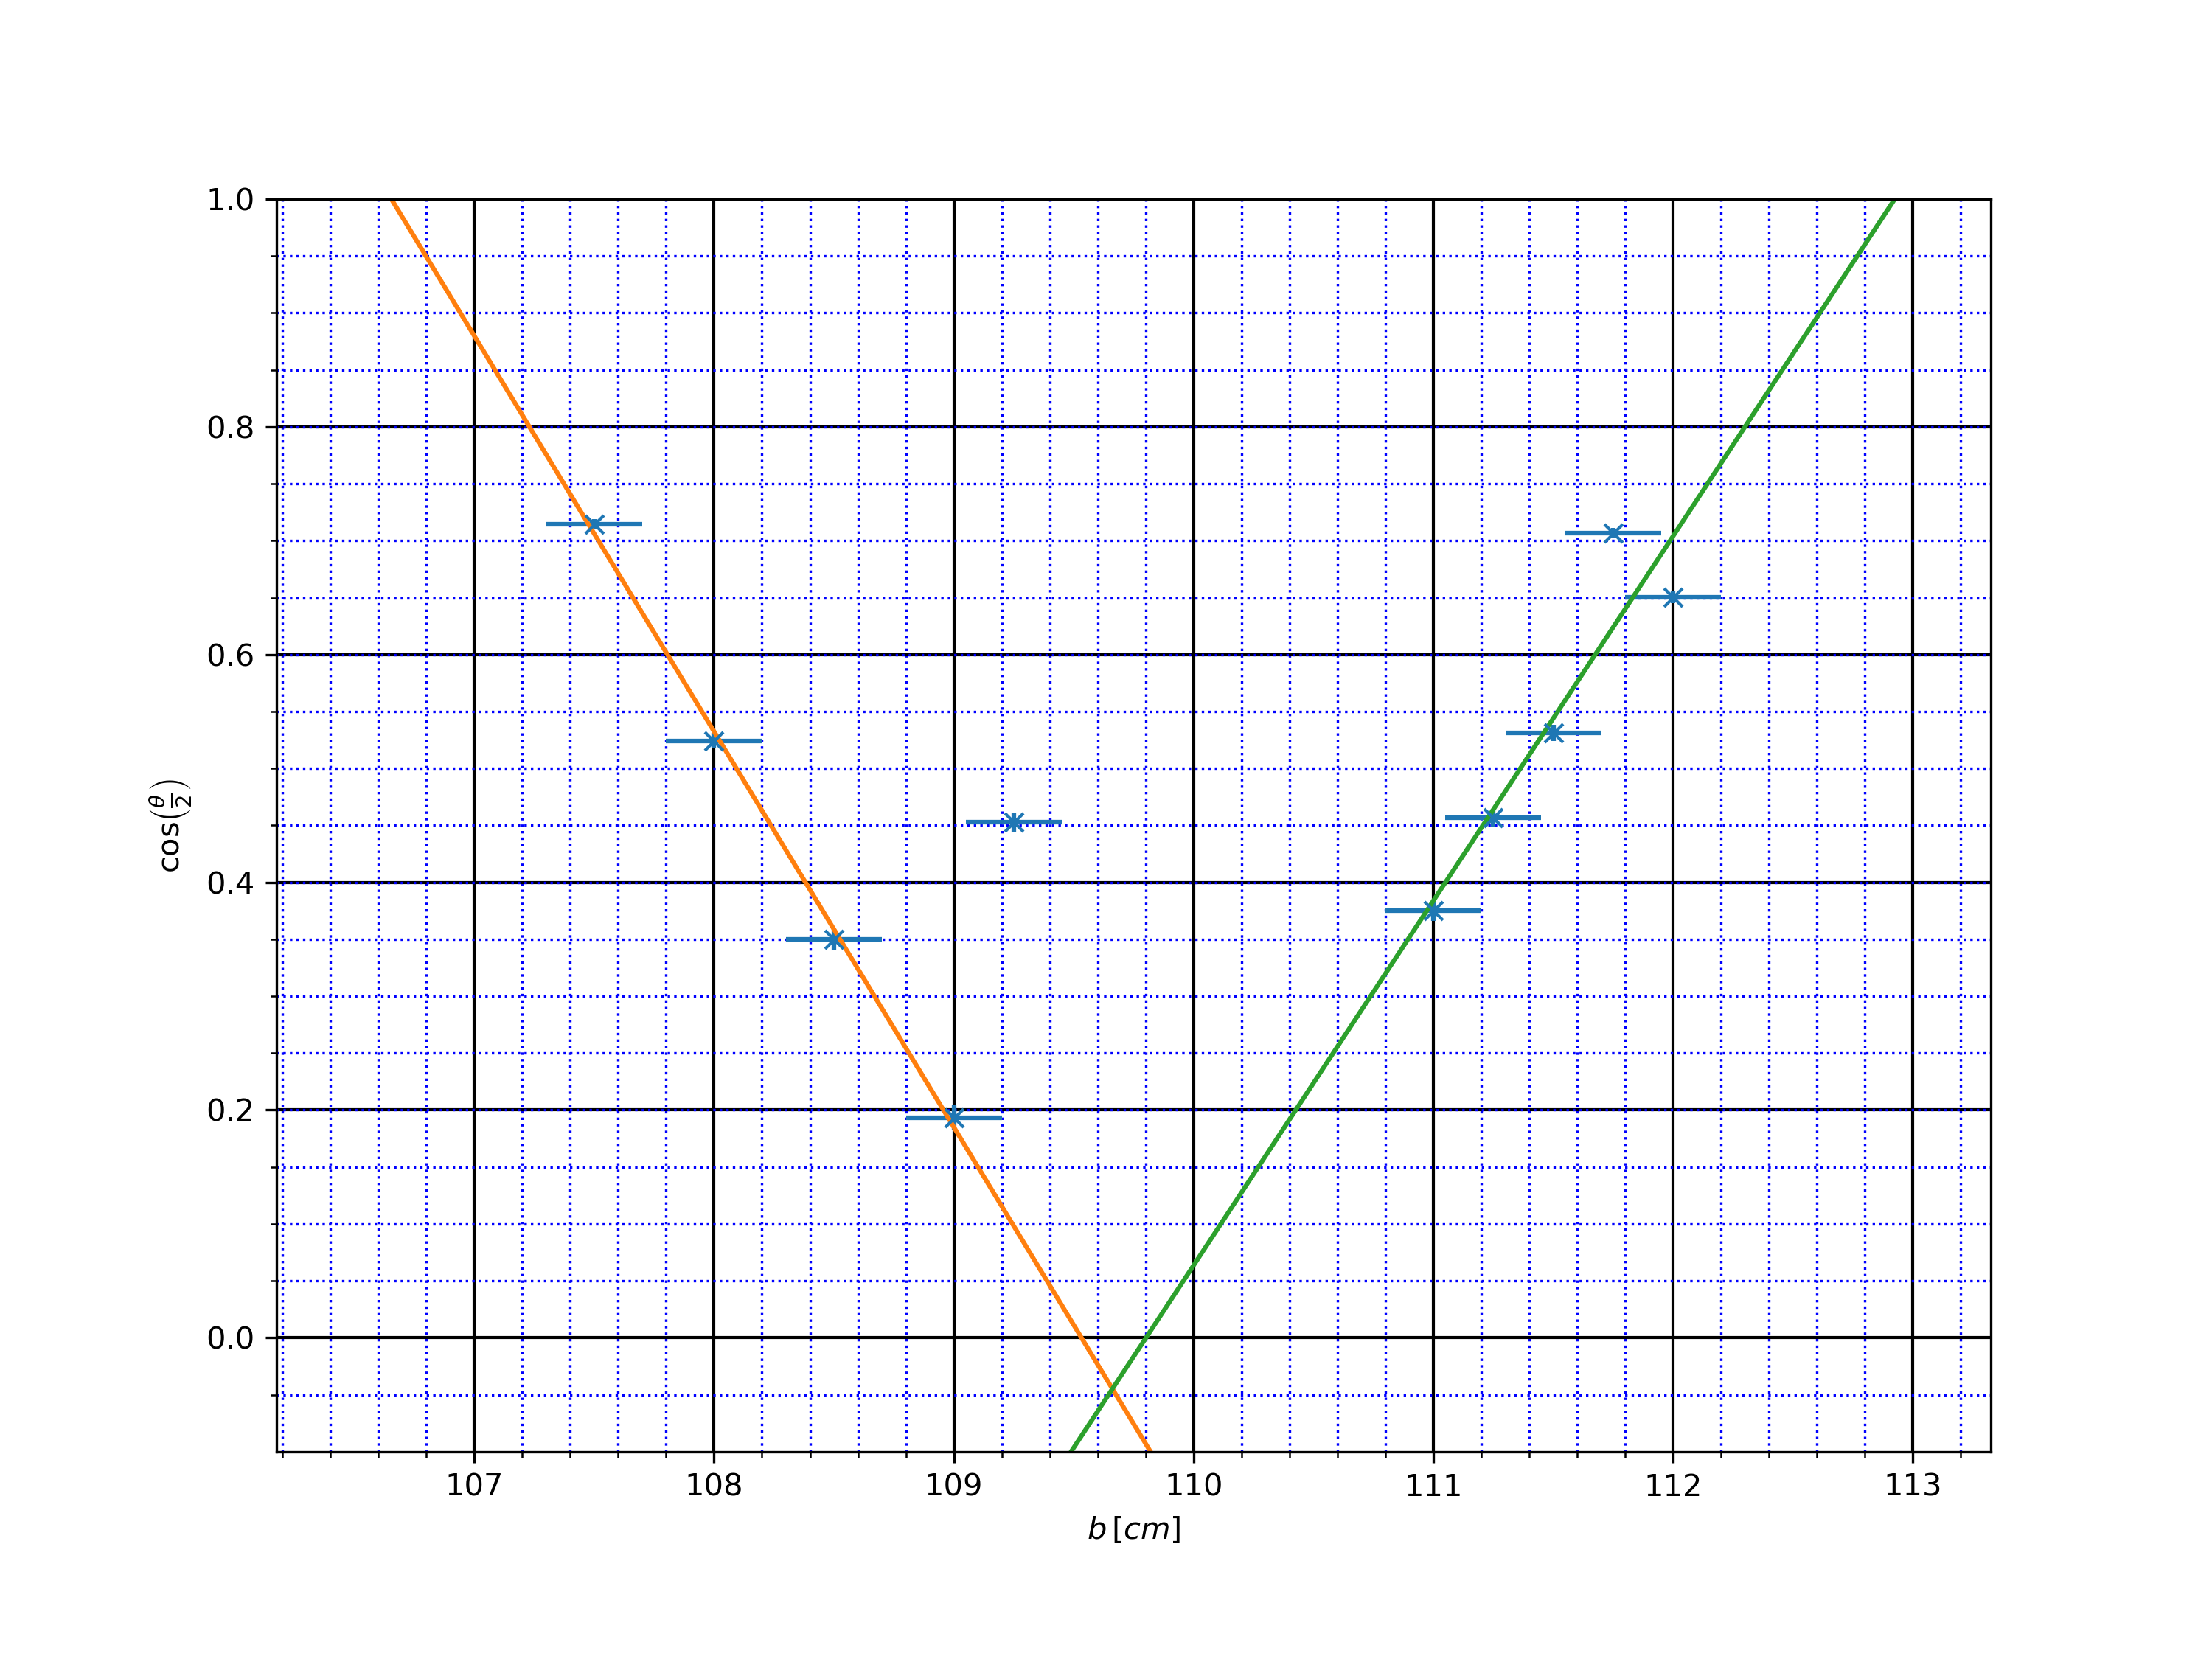
\includegraphics[width=0.8\textwidth]{graph.png}}
\renewcommand\thefigure{1}
\caption{Auftragung der Messwerte und lineare Regression. Der linke bzw. rechte Teil entspricht den Teil links bzw. rechts der Schu\ss apparatur.}
\label{Abb:1}
\end{figure}

Fehlerbalken in $y$-Achse sind hier schwer zu erkennen, wurden jedoch berechnet. Hierzu leiten wir $\cos\left(\frac{\theta}{2}\right)$ partiell nach $\theta$ ab:
\[
\frac{\partial\cos\left(\frac{\theta}{2}\right)}{\partial\theta}=-\frac{\sin\left(\frac{\theta}{2}\right)}{2}
\]

Der Betrag dieser partielle Ableitung mit dem Fehler von $\theta$ multipliziert ist also unser Fehler in der $y$-Achse.

Da unser Verlauch klar linear ist k\"onnen wir $\frac{1}{r+R}$ aus (\ref{eq:3}) der Steigung gleichsetzen. Wir rechnen also

\begin{equation}
\frac{1}{a}-r=R\label{eq:5}
\end{equation}

Da wir einen Fehler auf $a$ haben m\"ussen wir wieder gau\ss sche Fehlerfortpflanzung anwenden und erhalten

\[
\frac{\partial R}{\partial a}=-\frac{1}{a^2}
\]
\[
\Delta R=\left|\frac{\partial R}{\partial a}\Delta a\right|
\]

Mit unseren beiden Steigungen und dem vorgegebenen Radius der Kugeln, $2r=4.35\,\mathrm{mm}$, erhalten wir als Werte f\"ur den Radius unseres Targets:
\[r_1=2.66\pm0.09\]
\[r_2=2.9\pm0.7\]

Der Mittelwert hiervon mit (\ref{mean}) und (\ref{meanstd}) ist dann:

\[\bar{r}=2.8\pm0.4\]

\section{Diskussion}

Wollen wir die Korrektheit unserer Werte \"uberpr\"ufen, so ist leider kein Literaturwert vorhanden. Wir k\"onnen jedoch mit dem experimentell selbst gemessen Durchmesser vergleichen. Dieser Wert entspricht:
\[
d_r=(5.2\pm0.2)\,\mathrm{cm}
\]

Zum Vergleich verwenden wir folgende Formel:

\begin{equation}
t=\frac{\vert x_n-y_n\vert}{\sqrt{x_s^2+y_s^2}}\label{eq:6}
\end{equation}

Mit dieser Formel erhalten wir $t=0.005$. Dies impliziert, da es innerhalb des $t<2$ Bereichs ist, starke Vertr\"aglichkeit des Wertes. Jedoch haben wir einen sehr gro\ss en Fehler auf unser $\bar{r}$, n\"ahmlich entspricht dieser ca 14\%. Die Signifikanz des Wertes ist also nicht sehr hoch.

Ignorieren wir jedoch unseren Wert f\"ur $r_2$ und vergleichen einfach unser $r_1$ mittels (\ref{eq:6}), so erhalten wir
\[
t=0.006
\]
Zwar steigt unser $t$-Wert also leicht, jedoch haben wir eine wesentlich h\"ohere Signifikanz, da der Fehler nur noch 3\% des Ergebnisses ist.

Laut der guten \"Ubereinstimmung der gemessenen Ergebnisse k\"onnen wir also davon ausgehen, dass die theoretischen \"Uberlegungen sinnvoll sind.

Jedoch m\"ussen wir auch davon ausgehen, dass unser Experiment von systematischen Fehlern beeinflusst wurde. Ein Beispiel hierf\"ur ist, dass durchaus die M\"oglichkeit existiert, dass unsere Kugeln nicht alle mit der selben Geschwindigkeit und Ausrichtung gescho\ss en wurden. Die Apparatur k\"onnte sich w\"ahrend dem Nachladen leicht verschoben haben, da hierf\"ur der Bolzen rausgenommen werden musste und dann losgelassen wurde. Mit einer Feder hat sich der Bolzen dann zur\"uck bewegt. Der Einfluss dessen wird aber wohl nicht sehr gro\ss\ gewesen sein, da die $t$-Werte nicht sehr gro\ss\ sind.

Zur Verbesserung des Versuchs sollte eine gut Ablesbare Skala angebracht werden, damit $b$ leichter bestimmt werden kann. Au\ss erdem sollte man das Papier besser reinlegen, befestigen und den Mittelpunkt finden k\"onnen. Der Einfluss dieser Verbesserungen sollte aber nicht zu hoch sein, da diese eigentlich nur dazu dienen, dem Durchzuf\"uhrenden das Messen zu erleichtern.

Was jedoch einen gr\"o\ss eren Unterschied machen k\"onnte w\"are, wenn man eine Apparatur h\"atte, welche automatisch die Auftreffpunkte alle bestimmen w\"urde und deren Punkte einem geben w\"urde. Nat\"urlich ist dies aber zu zeitaufwendig zu erstellen, jedoch w\"aren dann die Mittelwerte der Auftreffpunkte genauer bestimmbar.

%\pagebreak
%
%\section{Anhang: Tabellen und Diagramme}
%
%\begin{table}[h]
%\centering
%\caption{XXXX} \vspace{11pt}
%$\begin{array}{l}
%\textrm{Unsicherheiten:}\\
%\textrm{XXXX: } \pm XX \textrm{XX}\\
%\end{array}$
%\begin{tabular}{ccc}
%\toprule
%\textrm{XXXX}/\textrm{XX} & \textrm{XXXX}/\textrm{XX} & \textrm{XXXX}/\textrm{XX} \\
%\midrule 
%2 & 0.26 & 0.23\\
%\hline
%4 & 0.33 & 0.25\\
%\hline 
%5 & & 0.3\\
%\hline 
%6 & 1.25 & 0.83\\
%\hline 
%8 & 3.9 & 0.83\\ 
%\hline
%9 & 4.75 & 4.6\\ 
%\hline
%10 & 4.7 &\\ 
%\bottomrule
%\end{tabular}
%\phantom{$\begin{array}{l}
%\textrm{Unsicherheiten:}\\
%\textrm{XXXX: } \pm XX \textrm{XX}\\
%\end{array}$}
%\label{Tab:X}
%\end{table}

%\begin{figure}[p]
%\centering
%\fbox{\includegraphics[width=0.8\textwidth]{NAME}}
%\renewcommand\thefigure{BX}
%\caption[XXXX]{XXXX}
%\label{Abb:X}
%\end{figure}

\begin{thebibliography}{9}
%\bibitem{Uncertainties}''Correlations between variables are automatically handled, which sets this module apart from many existing error propagation codes.'' - https://pythonhosted.org/uncertainties/
\bibitem{Anleitung} Physikalisches Institut der Albert-Ludwigs-Universität Freiburg (Hrsg.) (08/2018): Versuchsanleitungen zum Physiklabor für Anfänger*innen, Teil 1, Ferienpraktikum im Sommersemester 2018.
\end{thebibliography}

\end{document}